\documentclass[border=8pt]{standalone}
\usepackage[utf8]{vietnam}
\usepackage{times}
\usepackage{amsmath}
\usepackage{tikz}
\usetikzlibrary{arrows.meta}

\begin{document}
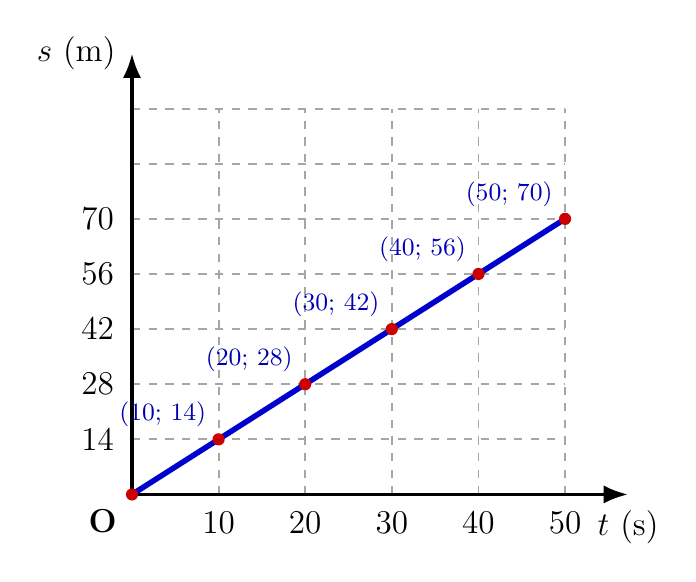
\begin{tikzpicture}[x=1cm, y=1cm, >=Latex, font=\large]
  % Grid
  \draw[dashed, line width=0.65pt, gray!70] (0,0) grid[xstep=1.1, ystep=0.7] (5.5,4.9);
  % Axes
  \draw[->, line width=1.3pt] (0,0) -- (6.3,0) node[below=2pt] {$t\text{ (s)}$};
  \draw[->, line width=1.3pt] (0,0) -- (0,5.6) node[left=2pt] {$s\text{ (m)}$};
  % Labels
  \node[below left=2pt] at (0,0) {\textbf{O}};
  \node[below=3pt] at (1.1,0) {10};
  \node[below=3pt] at (2.2,0) {20};
  \node[below=3pt] at (3.3,0) {30};
  \node[below=3pt] at (4.4,0) {40};
  \node[below=3pt] at (5.5,0) {50};
  
  \node[left=3pt] at (0,0.7) {14};
  \node[left=3pt] at (0,1.4) {28};
  \node[left=3pt] at (0,2.1) {42};
  \node[left=3pt] at (0,2.8) {56};
  \node[left=3pt] at (0,3.5) {70};
  
  % Points & Line
  \draw[line width=2.0pt, blue!80!black] (0,0) -- (5.5,3.5);
  \fill[red!80!black] (0,0) circle (2.2pt);
  \fill[red!80!black] (1.1,0.7) circle (2.2pt);
  \fill[red!80!black] (2.2,1.4) circle (2.2pt);
  \fill[red!80!black] (3.3,2.1) circle (2.2pt);
  \fill[red!80!black] (4.4,2.8) circle (2.2pt);
  \fill[red!80!black] (5.5,3.5) circle (2.2pt);
  
  % Label coordinates cleanly
  \node[above left=1pt, font=\small, blue!70!black] at (1.1,0.7) {(10; 14)};
  \node[above left=1pt, font=\small, blue!70!black] at (2.2,1.4) {(20; 28)};
  \node[above left=1pt, font=\small, blue!70!black] at (3.3,2.1) {(30; 42)};
  \node[above left=1pt, font=\small, blue!70!black] at (4.4,2.8) {(40; 56)};
  \node[above left=1pt, font=\small, blue!70!black] at (5.5,3.5) {(50; 70)};
\end{tikzpicture}
\end{document}
